\documentclass{beamer}
\usetheme{Luebeck}
\usecolortheme{seahorse}
\usefonttheme{structurebold,serif}
\setbeamertemplate{navigation symbols}{\usebeamerfont{footline}\insertframenumber/\inserttotalframenumber}
\usepackage[bold-style=ISO]{unicode-math}
\usepackage{luatexja-fontspec}
\setmainfont{DejaVu Serif}[Scale=0.9]
\setsansfont{DejaVu Sans}[Scale=0.9]
\setmonofont{DejaVu Sans Mono}[Scale=0.9]
\setmainjfont{YuKyo_Yoko-Medium}[BoldFont=YuKyo_Yoko-Bold]
\setsansjfont{YuGo-Medium}[BoldFont=YuGo-Bold]
\usepackage{hyperref}
\usepackage{graphicx}

\title{ペントミノ牧場パズル}
\author{宇佐見 公輔}
\date{2021年1月24日}
\begin{document}
\maketitle

\begin{frame}
    \frametitle{自己紹介}

    職業:プログラマ / 趣味:数学

    \bigskip

    最近の活動:
    \begin{itemize}
        \item ルービックキューブ群をSageMathで見る(10月 / 日曜数学会)
        \item ルービックキューブと群論(10月 / 関西日曜数学友の会)
        \item 平面の敷き詰めとルート系(6月 / 日曜数学会)
        \item 四元数のはなし(5月 / 関西日曜数学友の会)
    \end{itemize}
\end{frame}

\begin{frame}
    \frametitle{ペントミノ}

    正方形5つを辺どうしを合わせてつなげた形。
    回転・鏡像で重なるものを同じとみなすと、12個あります。

    \begin{figure}
        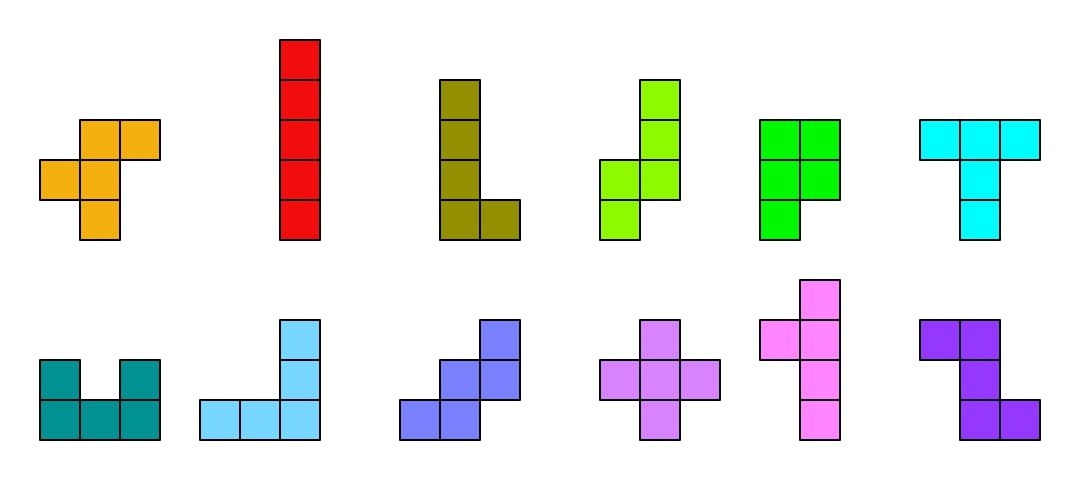
\includegraphics[scale=0.25]{images/Pentomino.png}
    \end{figure}
\end{frame}

\begin{frame}
    \frametitle{ペントミノパズル}

    ペントミノを使ったパズルとして、12個のピースを並べて平面図形を作る、というものがもっともよく知られています。

    次の図では、\(6 \times 10\) の長方形を作っています。

    \begin{figure}
        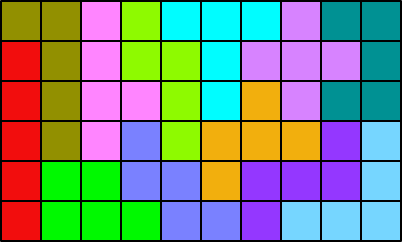
\includegraphics[scale=0.3]{images/PentominoTiling.png}
    \end{figure}
\end{frame}

\begin{frame}
    \frametitle{ペントミノパズルの解}

    一般的に「いくつかのポリオミノを使って特定の平面図形を作る」という問題に対して、それを解くアルゴリズムが知られています。
    (Donald E. Knuth, Dancing links, arXiv cs/0011047, 2000)

    \bigskip

    このアルゴリズムは SageMath に実装されていて、簡単に使うことができます。
    (sage.combinat.tiling.TilingSolver クラス)

    \bigskip

    先ほどの \(6 \times 10\) の長方形の場合、2339 通りの解があります。
\end{frame}

\begin{frame}
    \frametitle{ペントミノ牧場}

    ここでは、ペントミノを使った別のパズル、ペントミノ牧場(Pentomino farm)を紹介します。
    12個のピースを並べて輪を作ります。囲まれてできる図形の面積の最大値はいくつでしょうか。

    \begin{figure}
        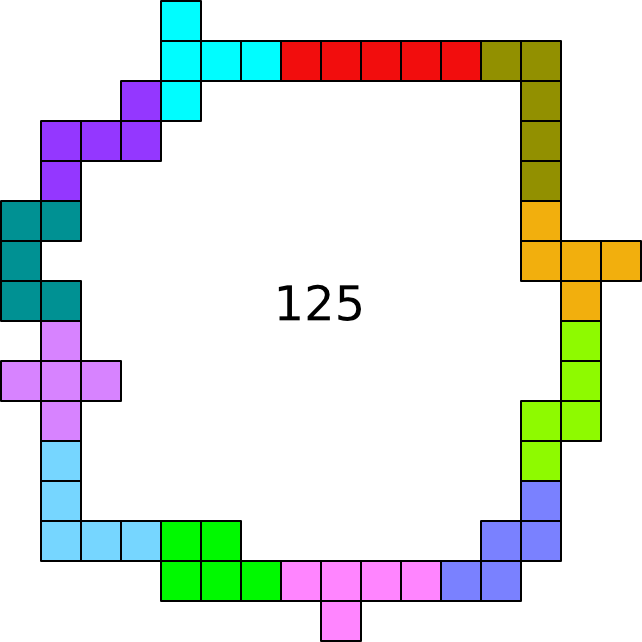
\includegraphics[scale=0.2]{images/PentominoFarm.png}
    \end{figure}
\end{frame}

\begin{frame}
    \frametitle{ペントミノ牧場の最大値}

    答えを示してしまいますが、最大値は128です。

    \bigskip

    ペントミノのタイリングパズルではコンピュータを使って解を出していました。
    そのため、ペントミノ牧場のパズルもコンピュータを使うのが良さそうに見えます。

    \bigskip

    しかし、実は理詰めで最大値が128であることを証明することができます。
    今回はその概略を説明します。
\end{frame}

\begin{frame}
    \frametitle{できる図形の形を考える}

    矩形を基準として内側にへこんだ形と考えることができます。

    \begin{figure}
        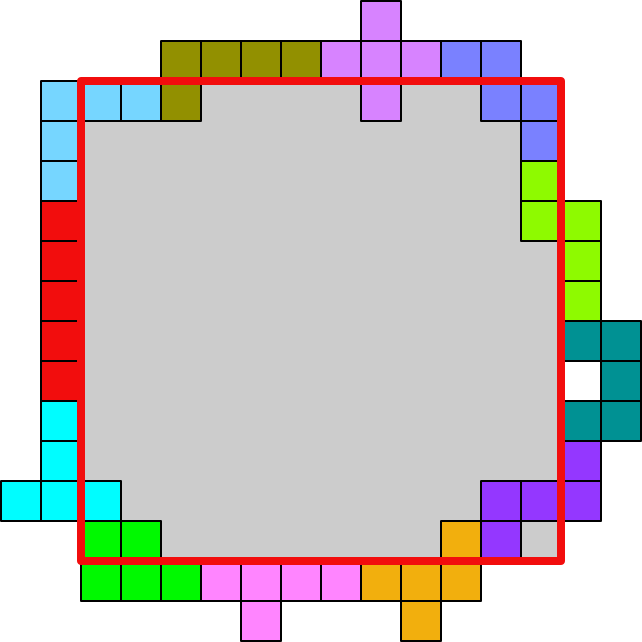
\includegraphics[scale=0.2]{images/PentominoFarmMax.png}
    \end{figure}

    矩形は \(12 \times 12 = 144\)、へこんだ部分は全部で \(17\)、飛び出ている部分が \(1\) です。
    したがって、\(144 - 17 + 1 = 128\) となります。
\end{frame}

\begin{frame}
    \frametitle{周の長さを考える (1)}

    可能な基準矩形の大きさを考えるために、周の長さを考えます。
    各ピースが周をかたちづくるときに、「他のピースから入ってくる正方形」と「他のピースに出ていく正方形」があります。
    その間の「長さ」の最大値がピースごとに決まります。

    \begin{figure}
        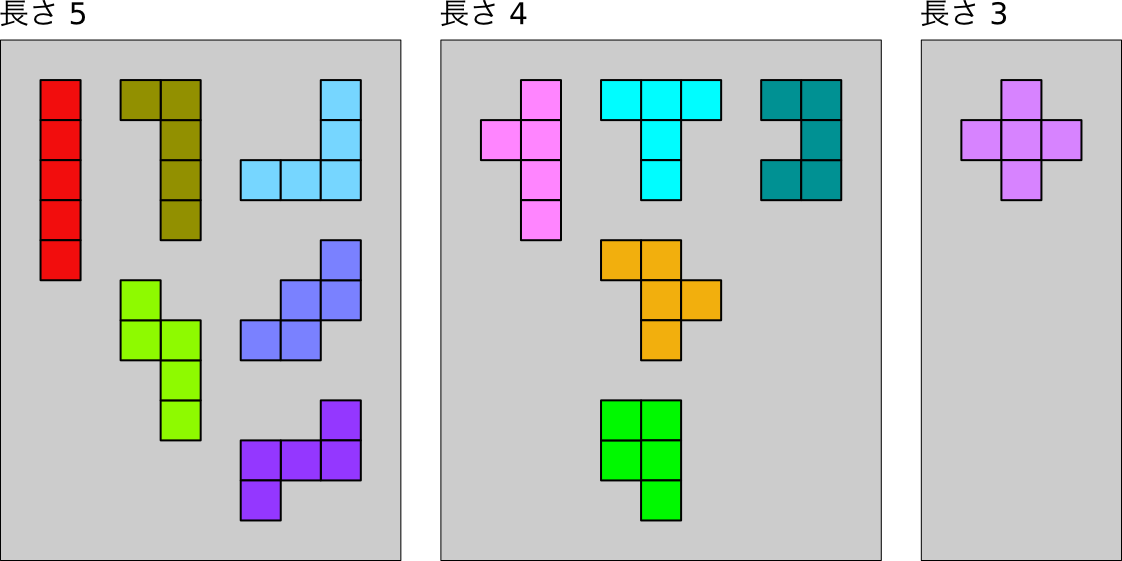
\includegraphics[scale=0.25]{images/PentominoFarmLength.png}
    \end{figure}
\end{frame}

\begin{frame}
    \frametitle{周の長さを考える (2)}

    合計すると \(5 \times 6 + 4 \times 5 + 3 \times 1 = 53\) です。
    矩形の周の長さなので偶数である必要があり、実際には \(52\) が最大です。

    \bigskip

    このことから、次のような矩形が基準として考えられます。

    \begin{itemize}
        \item \(13 \times 13\) の正方形 : 面積は \(12 \times 12 = 144\) です。
        \item \(14 \times 12\) の長方形 : 面積は \(13 \times 11 = 143\) です。
        \item \(15 \times 11\) の長方形 : 面積は \(14 \times 10 = 140\) です。
    \end{itemize}

    \bigskip

    1つのピースだけ最大の長さを使いません。
    U のピースを長さ 3 とみなして、矩形から飛び出る部分が 1 個生じると考えるのが最も効率が良いです。
\end{frame}

\begin{frame}
    \frametitle{ピースの分類}

    さらに突っ込んで考えるには「長さ」だけでなく、入ってから出るまでの「進み」と「寄り」で分類します。

    \begin{figure}
        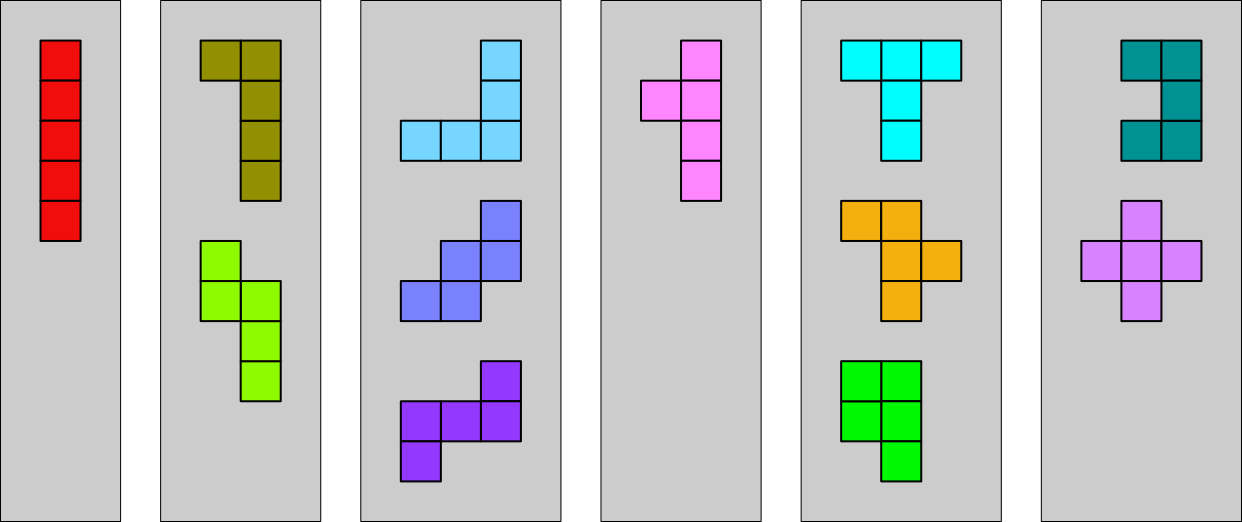
\includegraphics[scale=0.2]{images/PentominoFarmClass.png}
    \end{figure}
\end{frame}

\begin{frame}
    \frametitle{へこみの量}

    この分類から、基準矩形に対してへこみが \(6\) と飛び出しが \(1\) あることが分かります。

    \bigskip

    さらに細かく考えて、辺に置くべきピース、角に置くべきピースを考えると、基準矩形に対して \(11\) の削りが必要であることが分かります。

    \bigskip

    このため、\(144 - 6 + 1 - 11 = 128\) が最大面積であることが導けます。
\end{frame}

\begin{frame}
    \frametitle{参考文献}

    ペントミノパズル:

    \begin{itemize}
        \item Donald E. Knuth, \href{https://arxiv.org/abs/cs/0011047}{Dancing links}, arXiv cs/0011047
        \item \href{https://doc.sagemath.org/html/en/reference/combinat/sage/combinat/tiling.html}{Tiling Solver - Sage Reference Manual}
    \end{itemize}

    ペントミノ牧場:

    \begin{itemize}
        \item 島内剛一, \href{https://www.amazon.co.jp/dp/4535785376/ref=nosim?tag=usamik-22}{ルービック・キューブと数学パズル}
    \end{itemize}
\end{frame}

\end{document}
